\documentclass[11pt]{article}

\usepackage[margin=1in]{geometry}
\usepackage{amsmath,amssymb}
\usepackage{array}
\usepackage{booktabs}
\usepackage{caption}
\usepackage{float}
\usepackage{graphicx}
\usepackage{hyperref}
\usepackage{longtable}
\usepackage{xcolor}

\graphicspath{{../../artifacts/figures_static/}}
\hypersetup{
  colorlinks=true,
  linkcolor=blue!55!black,
  citecolor=blue!55!black,
  urlcolor=blue!55!black
}

\newcommand{\LIIS}{\mathrm{LIIS}}
\newcommand{\one}{\mathbf{1}}
\newcolumntype{L}[1]{>{\raggedright\arraybackslash}p{#1}}

\title{\textbf{Latent Insider Information Shocks}\\
\large Methodology, Variable Definitions, Data, and Empirical Results}
\author{Nima Taheri Hosseinkhani}
\date{June 2026}

\begin{document}
\maketitle

\begin{abstract}
This note documents the construction and empirical content of Latent Insider
Information Shocks (LIIS), a transaction-level measure designed to separate
economically informative insider filings from routine, planned, derivative-
linked, compensation-related, or mechanical Form 4 activity. The empirical
pipeline starts from WRDS Thomson Reuters Insiders, augments non-derivative
transactions with derivative-table, amendment, role, and 10b5-1 support fields,
and maps scored filings to CRSP PERMNO-month returns. The final production run
scores 17,328,988 insider transactions, maps 11,624,607 transaction rows into
the CRSP backtest, and produces a 390,627-row PERMNO-month LIIS panel over 203
monthly return periods. The main long-short portfolio formed on scaled LIIS earns
0.38 percent per month with a t-statistic of 1.94. The non-10b5 subset is
stronger, earning 0.42 percent per month with a t-statistic of 2.20. The evidence
supports a measurement interpretation: modern insider-filing information is not
well summarized by raw net buying or selling alone; it is concentrated in
transactions whose filing structure looks discretionary, material, and not
mechanical. The current evidence is promising but not yet a top-journal causal
claim; the Fama-MacBeth slope is weak in the current specification, and the
signal weakens sharply in the liquid-large robustness screen.
\end{abstract}

\section{Research Question and Contribution}

The economic question is whether insider filings contain priced information
after removing trades that are likely to be routine, pre-planned, derivative-
linked, tax-related, amendment-related, or compensation-driven. The question is
not whether insider trading can ever predict returns. That broad fact has a long
literature, including Lakonishok and Lee (2001) and Cohen, Malloy, and Pomorski
(2012). The sharper question is whether modern filing-level structure can
improve measurement of which individual Form 4 transactions should count as
information-bearing signals.

The project therefore treats insider filings as a measurement problem before it
treats them as an asset-pricing signal. A raw Form 4 transaction is first
converted into a transaction-level probability of being informative. The
probability is learned from filing characteristics that distinguish open-market
and material transactions from mechanical or planned transactions. These
transaction scores are then aggregated into firm-month state variables and tested
against future stock returns. This design is closest in spirit to the routine
versus opportunistic distinction in Cohen, Malloy, and Pomorski (2012), but it
differs in the unit of classification and in the information set: the object here
is a transaction-level score that incorporates derivative companions, amendments,
10b5-1 indicators, filing lags, role information, and missingness structure.

The contribution is best stated as a measurement and implementation claim:
modern insider filings contain useful return-relevant information, but the
information is concentrated in transactions that survive a richer filing-structure
filter. The strongest current evidence is the non-10b5 and amendment-strict
portfolio evidence. The weakest current evidence is the monthly cross-sectional
Fama-MacBeth slope, which does not yet support a broad characteristic-pricing
claim.

\section{Data}

The production run uses the following data sources.

\begin{longtable}{L{0.23\linewidth}L{0.31\linewidth}L{0.36\linewidth}}
\caption{Data Inputs and Use in the LIIS Pipeline}\label{tab:data_inputs}\\
\toprule
\textbf{Source} & \textbf{Tables or Files} & \textbf{Use}\\
\midrule
\endfirsthead
\toprule
\textbf{Source} & \textbf{Tables or Files} & \textbf{Use}\\
\midrule
\endhead
WRDS Thomson Reuters Insiders &
Non-derivative Table 1; derivative Table 2; filing headers; 10b5-1 support;
amendment support; company support &
Defines insider transactions, filing dates, transaction dates, transaction
codes, roles, ownership, 10b5-1 indicators, amendment links, and derivative
companions.\\
\addlinespace
CRSP monthly stock file &
Monthly returns, prices, shares outstanding, market capitalization, and
security identifiers &
Maps LIIS to future stock returns and scales firm-month signals by lagged or
current market capitalization.\\
\addlinespace
CRSP daily stock file &
Daily returns around filing dates &
Constructs event-time return paths around filing availability.\\
\addlinespace
CRSP names history &
PERMNO, CUSIP, NCUSIP, share code, and valid name dates &
Builds a date-valid CUSIP6-month to PERMNO bridge for insider transactions.\\
\addlinespace
CRSP/Compustat Merged and Compustat &
CCM link history; annual and quarterly fundamentals &
Provides accounting and identifier support for the broader research design.
The current headline tests use CRSP return joins and market-cap controls.\\
\addlinespace
Kenneth French factor files &
Monthly Fama-French three-factor series &
Provides factor-loadings diagnostics for the LIIS long-short return.\\
\addlinespace
TAQ entitlement probe &
TAQ candidate schemas and small-access checks &
TAQ schemas were visible, but sample queries returned permission errors. TAQ is
therefore not used in the reported implementation-cost calibration.\\
\bottomrule
\end{longtable}

The intended insider sample window is January 2004 through December 2025, with
2026 reserved as a future holdout. The realized return panel starts later after
identifier mapping and return availability filters. The final backtest contains
203 monthly return periods and 390,627 PERMNO-month observations. All sample
counts and coefficients in this note are taken from the current run manifests
and summary tables, while all variable definitions are taken from the current
pipeline code.

\section{Transaction-Level Construction}

Let $j$ index an insider transaction, $i(j)$ the issuing firm, and $f_j$ the
filing date on which the transaction becomes available in the insider-filing
data. Let $\tau_j$ denote the transaction date, $q_j$ the reported share amount,
$p^{\mathrm{price}}_j$ the reported transaction price, and $a_j$ the acquired-
or-disposed indicator. The trade sign is
\begin{equation}
s_j =
\begin{cases}
+1, & a_j=A \text{ or transaction code in } \{P,A\},\\
-1, & a_j=D \text{ or transaction code in } \{S,D\},\\
\mathrm{missing}, & \text{otherwise.}
\end{cases}
\end{equation}
The signed and absolute dollar values are
\begin{equation}
V_j = s_j |q_j| |p^{\mathrm{price}}_j|,\qquad |V_j|=|V_j|.
\end{equation}
The filing lag is
\begin{equation}
\ell_j = f_j-\tau_j,
\end{equation}
measured in calendar days. In the predictive feature vector, the lag is clipped
to the interval $[-30,365]$, with missing lags assigned a separate large value.

Transaction code families are defined from the Form 4 code. Open-market trades
are codes $P$ and $S$. Mechanical-code transactions include grants or awards,
option or derivative exercises, tax or disposition codes, gifts, and other
non-standard code families. The indicator for a mechanical transaction is
\begin{align}
M_j ={}&
\one\{\text{grant or award}\}
\vee \one\{\text{option or derivative code}\} \nonumber\\
&\vee \one\{\text{tax or disposition code}\}
\vee \one\{\text{gift or other code}\}.
\end{align}
Role indicators identify CEO/CFO, director, and officer language in the reporting
person title or role-code fields. The 10b5-1 flag is constructed from both the
main transaction record and the support table. Derivative companions are
identified by grouping derivative Table 2 records by filing accession, person,
and security identifiers. Let $D_j$ be the derivative companion count. The
indicator
\begin{equation}
H^{\mathrm{deriv}}_j=\one\{D_j>0\}
\end{equation}
marks transactions that have at least one derivative companion record.
Amendment status is identified from amendment support tables or, when the
support table is absent, from the amendment flag in the main insider record.

The routine-or-mechanical flag is
\begin{equation}
R_j = M_j \vee B^{10b5}_j \vee H^{\mathrm{deriv}}_j \vee A^{\mathrm{amend}}_j,
\end{equation}
where $B^{10b5}_j$ is the 10b5-1 indicator and $A^{\mathrm{amend}}_j$ marks an
amended record. The transaction-level weak label used for model training is
\begin{equation}
Y_j =
\one\{\text{open-market}_j\}
\cdot
\one\{B^{10b5}_j=0\}
\cdot
\one\{R_j=0\}
\cdot
\one\{|V_j|>Q_{0.60}(|V|)\}.
\end{equation}
This label is not a legal definition of informed trading. It is a noisy
supervision device: large, open-market, non-10b5, non-mechanical transactions
are treated as candidate informative events, while routine or mechanical
transactions are downweighted.

\section{Predictive Model and Score}

The transaction-level feature vector $X_j$ includes
\begin{align}
X_j = (&\log(1+|V_j|),\; \ell^{\mathrm{clip}}_j,\;
\log(1+\min\{1000, |q_j|/|h_j|\}),\; \log(1+D_j),\\
&\one\{f_j \geq \mathrm{April\ 1,\ 2023}\},\;
\one\{\text{open-market}\},\; M_j,\; B^{10b5}_j,\;
\one\{\text{CEO/CFO}\},\\
&H^{\mathrm{deriv}}_j,\; A^{\mathrm{amend}}_j,\;
\one\{\text{missing price}\},\; \one\{\text{missing shares}\},\\
&\one\{\text{tax or disposition code}\},\;
\one\{\text{option or derivative code}\}).
\end{align}
Here $h_j$ is shares held after the transaction when available. The 2023
indicator reflects the modern 10b5-1 disclosure era after the SEC's 2022
amendments to insider-trading plan disclosures.

Three model families are estimated. First, rules-only scoring provides a
transparent baseline. Second, Elastic Net logistic regression provides a sparse
linear benchmark. Third, a LightGBM classifier provides the main tabular model.
A PyTorch neural-network branch is trained on the same transaction-level
features as a GPU extension. The final score is a blend:
\begin{equation}
\widehat{p}_j =
0.70\,\widehat{p}^{\mathrm{LGBM}}_j
+0.30\,\widehat{p}^{\mathrm{MLP}}_j.
\end{equation}
In the production environment, LightGBM's GPU tree learner was unavailable in
the installed build, so the LightGBM branch ran on CPU. The PyTorch branch did
use the A100 GPU and trained on 3,000,000 transaction rows for three epochs.

The transaction-level signed information value is
\begin{equation}
Z_j = s_j \widehat{p}_j |V_j|.
\end{equation}
This object is positive for predicted-informative purchases, negative for
predicted-informative sales, and close to zero for small or low-probability
transactions.

\section{Firm-Month LIIS Variables}

Let $\mathcal{J}_{i,t}$ be the set of insider transactions for firm $i$ filed in
month $t$ and mapped to a valid CRSP PERMNO. The main firm-month signal is
\begin{equation}
\LIIS^{\mathrm{net}}_{i,t} =
\sum_{j\in\mathcal{J}_{i,t}} Z_j.
\end{equation}
The buy and sell components are
\begin{equation}
\LIIS^{\mathrm{buy}}_{i,t} =
\sum_{j\in\mathcal{J}_{i,t}} Z_j \one\{Z_j>0\},\qquad
\LIIS^{\mathrm{sell}}_{i,t} =
\sum_{j\in\mathcal{J}_{i,t}} Z_j \one\{Z_j<0\}.
\end{equation}
Role- and mechanism-specific variants are constructed by applying indicator
filters before aggregation:
\begin{align}
\LIIS^{\mathrm{CEO/CFO}}_{i,t} &=
\sum_{j\in\mathcal{J}_{i,t}} Z_j \one\{\text{CEO/CFO}_j\},\\
\LIIS^{\mathrm{nonplan}}_{i,t} &=
\sum_{j\in\mathcal{J}_{i,t}} Z_j \one\{B^{10b5}_j=0\},\\
\LIIS^{\mathrm{open}}_{i,t} &=
\sum_{j\in\mathcal{J}_{i,t}} Z_j \one\{\text{open-market}_j\},\\
\LIIS^{\mathrm{amend-strict}}_{i,t} &=
\sum_{j\in\mathcal{J}_{i,t}} Z_j \one\{A^{\mathrm{amend}}_j=0\}.
\end{align}
Each signal is scaled by market capitalization:
\begin{equation}
\widetilde{\LIIS}_{i,t} =
\frac{\LIIS^{\mathrm{net}}_{i,t}}{\mathrm{MCap}_{i,t-1}},
\end{equation}
using lagged market capitalization when available and current market
capitalization otherwise. The scaled variables enter portfolio sorts and
cross-sectional regressions.

The portfolio construction sorts stocks into deciles within each month using
$\widetilde{\LIIS}_{i,t}$. The long-short return is
\begin{equation}
R^{10-1}_{t+1} =
\frac{1}{N_{10,t}}\sum_{i\in D_{10,t}} R_{i,t+1}
-
\frac{1}{N_{1,t}}\sum_{i\in D_{1,t}} R_{i,t+1}.
\end{equation}
Cumulative performance is computed as $\prod_{\tau\leq t}(1+R^{10-1}_{\tau})-1$.

The Fama-MacBeth-style cross-sectional regression is
\begin{equation}
R_{i,t+1} =
\alpha_t + \beta_t \widetilde{\LIIS}_{i,t}
+ \gamma_t \log(\mathrm{MCap}_{i,t})+\varepsilon_{i,t+1},
\end{equation}
estimated separately by month. The reported slope is the time-series mean of
$\beta_t$ divided by its time-series standard error. Factor diagnostics estimate
\begin{equation}
R^{10-1}_{t}=\alpha+\beta_M \mathrm{MKT}_t+\beta_S\mathrm{SMB}_t+
\beta_H\mathrm{HML}_t+\eta_t
\end{equation}
against monthly Fama-French three-factor returns.

\section{Variable Glossary}

\begin{longtable}{L{0.30\linewidth}L{0.60\linewidth}}
\caption{Main Variables Created by the Pipeline}\label{tab:glossary}\\
\toprule
\textbf{Variable} & \textbf{Definition}\\
\midrule
\endfirsthead
\toprule
\textbf{Variable} & \textbf{Definition}\\
\midrule
\endhead
$s_j$ & Transaction sign. Purchases/acquisitions are $+1$; sales/dispositions
are $-1$.\\
$V_j$ & Signed dollar value, $s_j |q_j||p^{\mathrm{price}}_j|$.\\
$|V_j|$ & Absolute transaction dollar value.\\
$\ell_j$ & Filing lag in days, filing date minus transaction date.\\
\texttt{is\_open\_market} & Indicator for open-market purchase or sale codes
$P$ and $S$.\\
\texttt{is\_mechanical\_code} & Indicator for grant, award, derivative exercise,
tax-withholding, gift, or other mechanical transaction-code families.\\
\texttt{is\_10b5} & Indicator that the transaction is marked as related to a
10b5-1 plan in the main or support table.\\
\texttt{has\_derivative\_\allowbreak companion} & Indicator that derivative
Table 2 contains at least one companion record linked to the same
filing/person/security combination.\\
\texttt{is\_amended\_record} & Indicator that the transaction belongs to or is
linked to an amendment record.\\
$R_j$ & Routine-or-mechanical flag combining mechanical codes, 10b5-1 status,
derivative companions, and amendment status.\\
$Y_j$ & Weak informative label for model training: large open-market,
non-10b5, non-routine transactions.\\
$\widehat{p}_j$ & Predicted probability that transaction $j$ is economically
informative.\\
$Z_j$ & Signed information value, $s_j \widehat{p}_j |V_j|$.\\
$\LIIS^{\mathrm{net}}_{i,t}$ & Sum of $Z_j$ across transactions filed by firm
$i$ in month $t$.\\
$\widetilde{\LIIS}_{i,t}$ & Market-cap-scaled net LIIS.\\
$\LIIS^{\mathrm{nonplan}}_{i,t}$ & LIIS using only transactions without a
10b5-1 indicator.\\
$\LIIS^{\mathrm{amend-strict}}_{i,t}$ & LIIS excluding amended records.\\
\texttt{liis\_cluster} & Maximum of distinct buy-side and sell-side insider
owner counts in a firm-month.\\
\texttt{liis\_disagreement} & Entropy-style disagreement measure based on the
share of distinct buy-side versus sell-side owners.\\
$R^{10-1}_{t+1}$ & Equal-weight return of LIIS decile 10 minus LIIS decile 1 in
the next month.\\
\bottomrule
\end{longtable}

The owner-count variables are included because the pipeline creates them for
cluster and disagreement diagnostics. In the current mapped panel, the owner
count fields do not contribute meaningful variation, so they should not be used
as evidence for the headline result until the owner identifier feed is audited.

\section{Empirical Results}

\subsection{Transaction scoring and model interpretation}

The model-training run scores 17,328,988 transactions and uses 13,639,115
transactions in the training window. Elastic Net logistic regression completes
successfully, the LightGBM tabular model completes on CPU, and the PyTorch GPU
MLP branch completes on the A100. Table~\ref{tab:model_variants} summarizes the
model status.

\begin{table}[H]
\centering
\caption{Model Variants}
\label{tab:model_variants}
\begin{tabular}{L{0.24\linewidth}L{0.31\linewidth}L{0.32\linewidth}}
\toprule
Model & Role & Status\\
\midrule
Rules only & Transparent baseline & Available\\
Elastic Net logistic & Sparse benchmark & Ok\\
LightGBM & Main tabular workhorse & Ok, CPU tree learner\\
Torch GPU MLP & GPU sequence/tabular extension & Ok\\
Blend & Production score & LightGBM CPU plus torch GPU MLP\\
\bottomrule
\end{tabular}
\end{table}

The SHAP summary in Figure~\ref{fig:shap} indicates that the most important
stage-one inputs are absolute dollar value, open-market status, and derivative
companion structure. This interpretation is economically coherent: the score
puts weight on material discretionary trades and discounts transactions that
look mechanical or derivative-linked.

\begin{figure}[H]
\centering
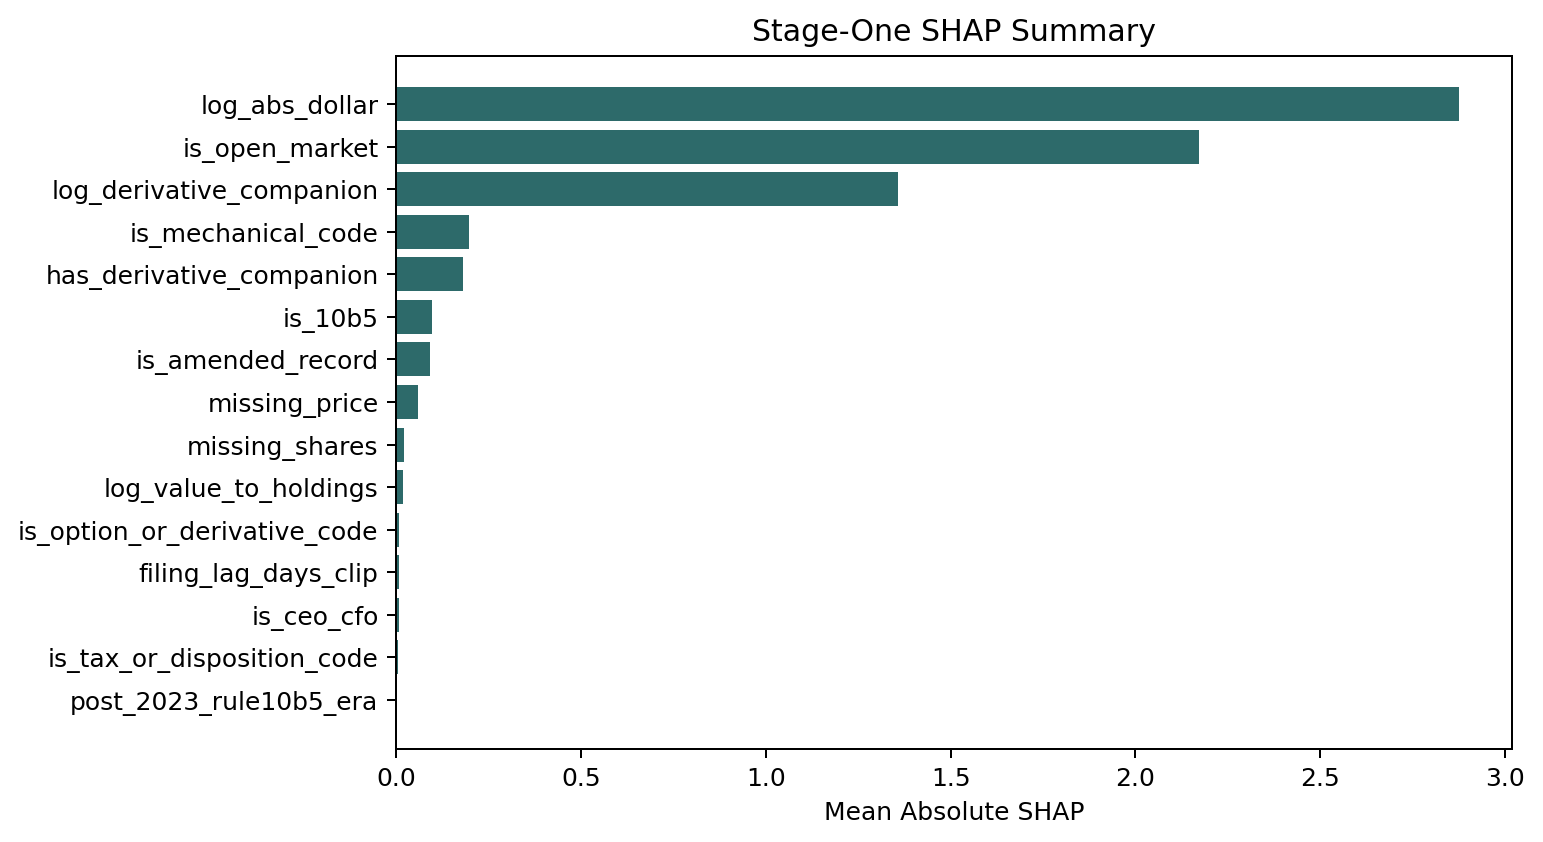
\includegraphics[width=0.92\linewidth]{fig_shap_summary.png}
\caption{Stage-One SHAP Summary. The figure reports mean absolute SHAP values
for the LightGBM stage-one model.}
\label{fig:shap}
\end{figure}

\subsection{Portfolio returns}

The main LIIS decile portfolio produces 203 monthly long-short returns. The
average monthly return is 0.35 percent in the realized decile table and 0.38
percent in the robustness recomputation, with a robustness t-statistic of 1.94.
The approximate annual return is 4.26 percent, the annual volatility is 9.87
percent, and the approximate Sharpe ratio is 0.43. The maximum drawdown is
$-25.63$ percent.

\begin{table}[H]
\centering
\caption{Performance Summary}
\label{tab:performance}
\begin{tabular}{L{0.36\linewidth}rrrr}
\toprule
Series & Months & Mean monthly & Annual return & Annual vol.\\
\midrule
Long-short decile 10 minus decile 1 & 203 & 0.00355 & 0.04258 & 0.09873\\
\bottomrule
\end{tabular}
\end{table}
The maximum drawdown for this series is $-25.63$ percent.

\begin{figure}[H]
\centering
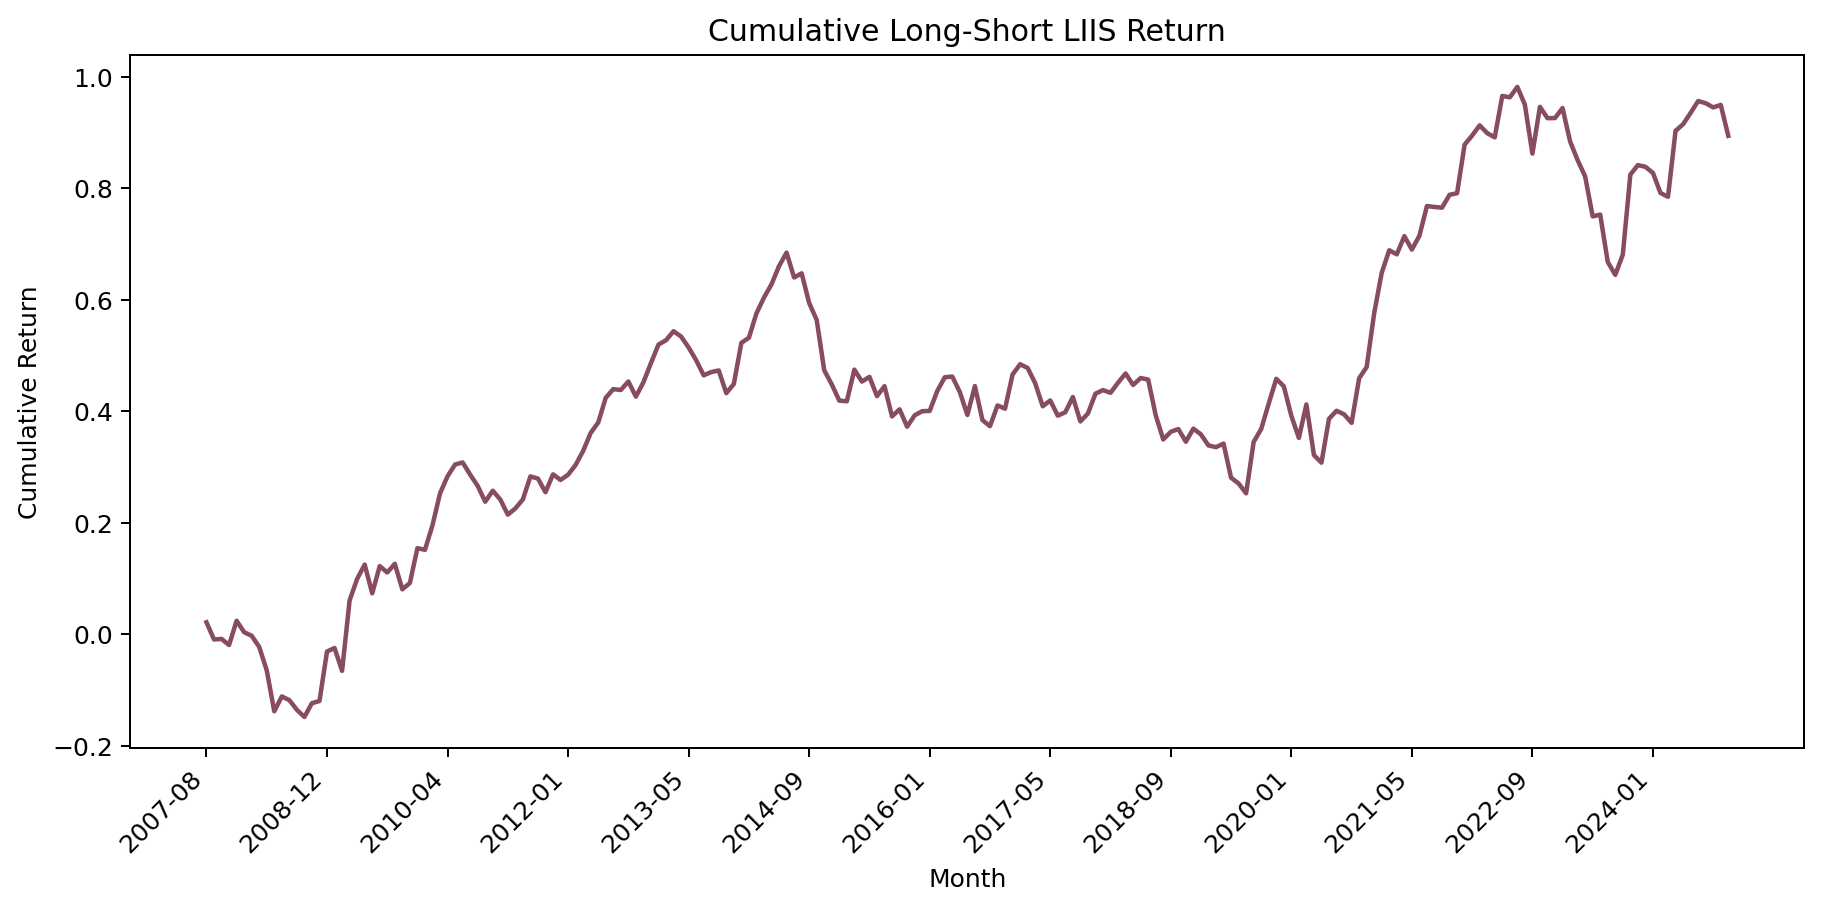
\includegraphics[width=0.92\linewidth]{fig_cumulative_pnl_gross_net.png}
\caption{Cumulative Long-Short LIIS Return. The line plots cumulative wealth
from the equal-weight decile 10 minus decile 1 return.}
\label{fig:cumulative}
\end{figure}

\begin{figure}[H]
\centering
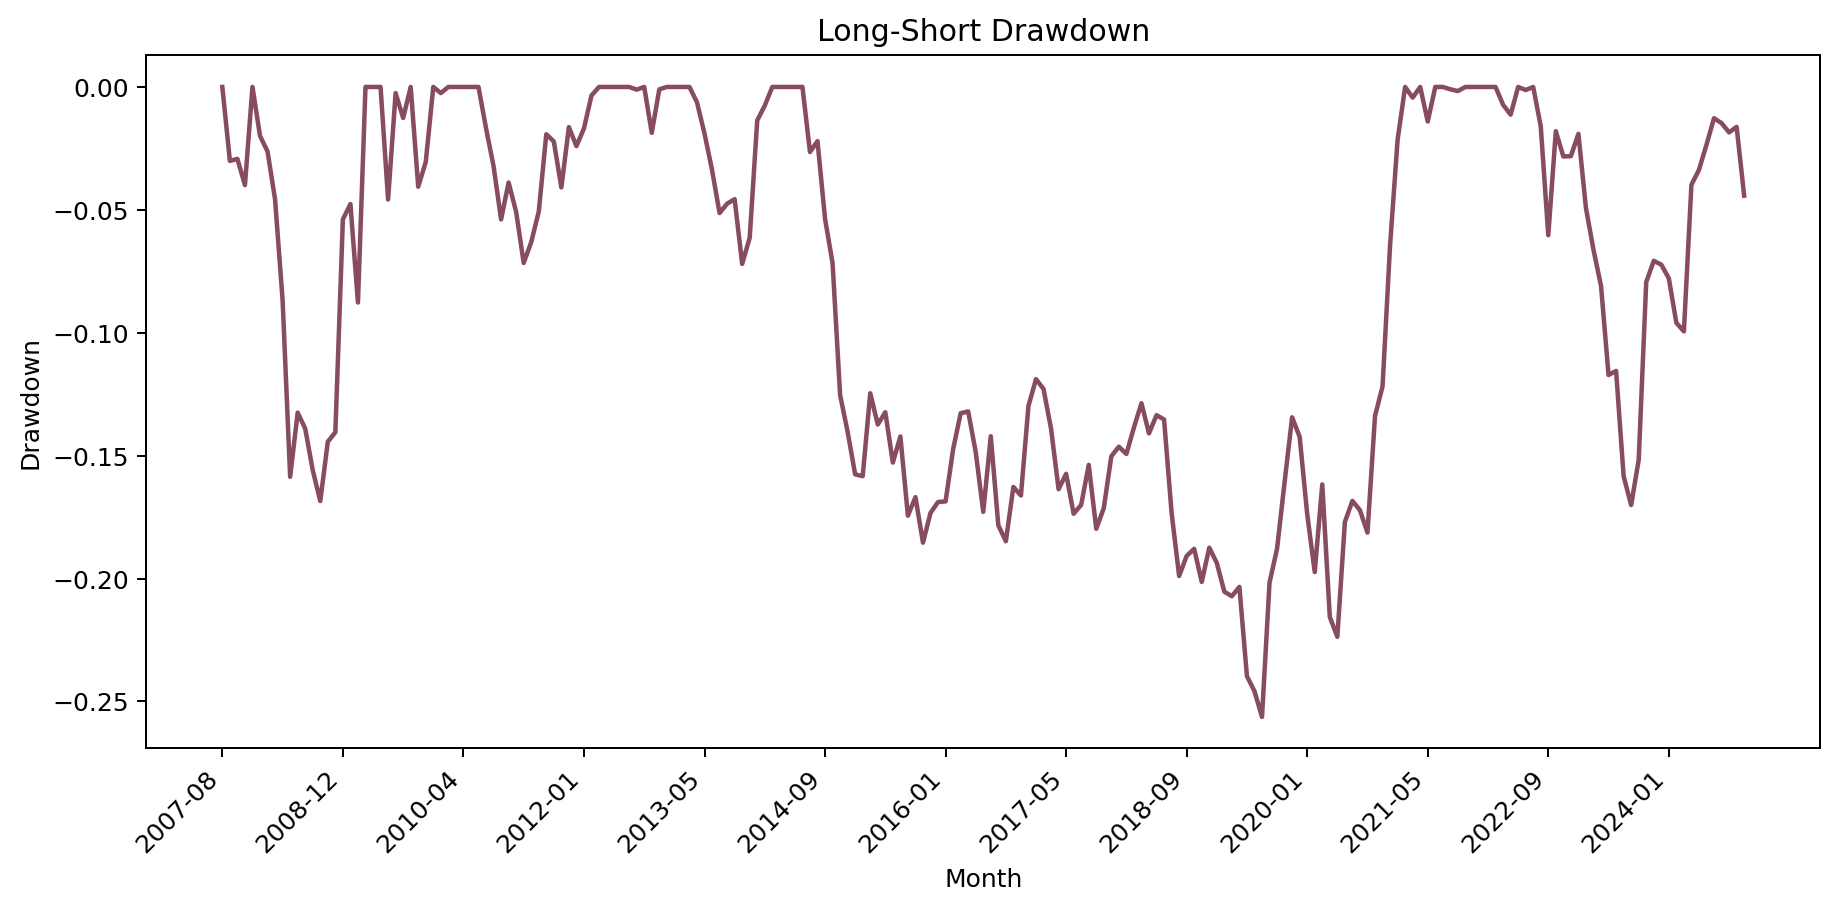
\includegraphics[width=0.92\linewidth]{fig_drawdown_turnover.png}
\caption{Long-Short Drawdown. The figure reports drawdowns for the same
long-short return series.}
\label{fig:drawdown}
\end{figure}

\subsection{Robustness}

Table~\ref{tab:robustness} reports the robustness battery. The strongest
variant is the non-10b5 signal, with a mean monthly long-short return of 0.42
percent and a t-statistic of 2.20. The amendment-strict version is close to the
main signal, with a t-statistic of 1.92. The open-market-only version remains
positive but weaker. The liquid-large screen is weak, which is an important
scope condition for publication claims and implementation interpretation.

\begin{table}[H]
\centering
\caption{Robustness Summary}
\label{tab:robustness}
\begin{tabular}{lrrr}
\toprule
Test & Months & Mean long-short & t-statistic\\
\midrule
Main LIIS net & 203 & 0.00380 & 1.94\\
Buys only & 203 & 0.00217 & 1.23\\
Sells only & 203 & -0.00060 & -0.31\\
CEO/CFO only & 203 & 0.00221 & 1.12\\
Non-10b5 only & 203 & 0.00424 & 2.20\\
Open-market only & 203 & 0.00282 & 1.50\\
Amendment strict & 203 & 0.00381 & 1.92\\
Liquid-large 70 percent & 203 & 0.00019 & 0.09\\
Placebo shuffle within month & 203 & 0.00134 & 1.28\\
Transaction-date alignment & 251 & 0.00484 & 2.88\\
\bottomrule
\end{tabular}
\end{table}

\subsection{Event-time validation}

The event-time validation groups filing-date events by the event-level LIIS
score and computes cumulative average daily returns over business days $-5$ to
$+5$ around filing availability. The current event-time exhibit uses CRSP daily
returns and should be interpreted as an event-time return validation rather than
a fully benchmark-adjusted abnormal-return design. The run includes 939,844
event-window observations across 10 event deciles.

\begin{figure}[H]
\centering
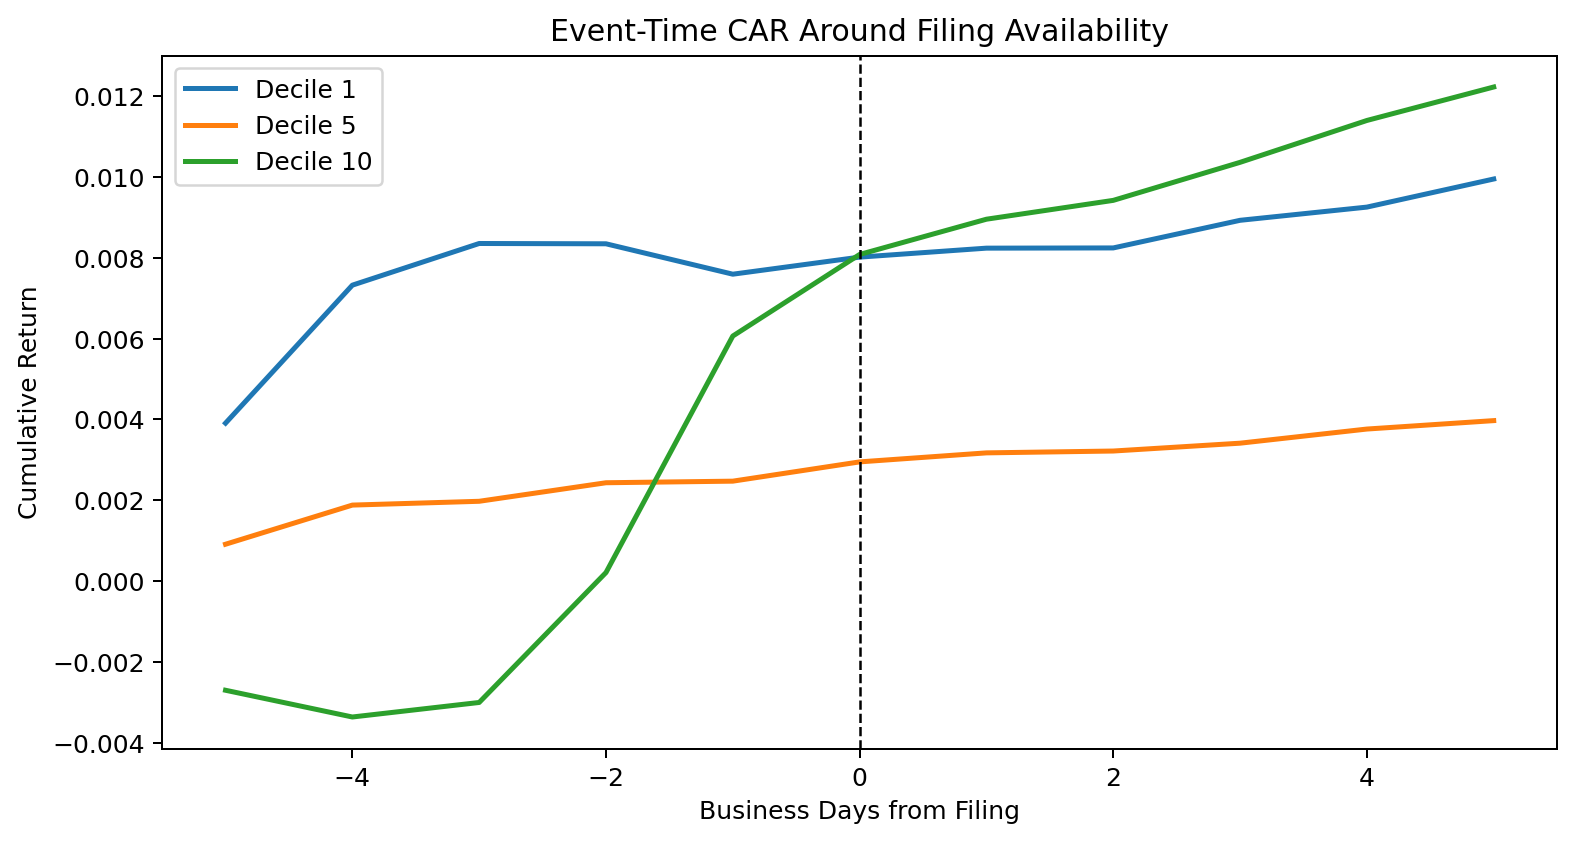
\includegraphics[width=0.92\linewidth]{fig_event_car_by_decile.png}
\caption{Event-Time Cumulative Returns Around Filing Availability. The figure
plots selected LIIS event deciles from business days $-5$ to $+5$.}
\label{fig:event}
\end{figure}

\subsection{Factor and cross-sectional pricing diagnostics}

The factor-loading diagnostic regresses the LIIS long-short return on the
Fama-French market, SMB, and HML factors. The estimated monthly intercept is
0.36 percent over 203 months. The market loading is small, while the HML loading
is positive.

\begin{table}[H]
\centering
\caption{Fama-French Factor Loading Diagnostic}
\label{tab:factors}
\begin{tabular}{lrr}
\toprule
Term & Loading & Months\\
\midrule
Alpha & 0.00361 & 203\\
Mkt-RF & 0.01103 & 203\\
SMB & 0.03633 & 203\\
HML & 0.10474 & 203\\
\bottomrule
\end{tabular}
\end{table}

The current Fama-MacBeth-style cross-sectional diagnostic is weaker. The
time-series mean coefficient on scaled LIIS is $-0.0070$ with a t-statistic of
$-0.28$ over 203 months. This result argues against making a broad
characteristic-pricing claim at this stage. The portfolio evidence is promising,
but a top-journal version of the paper should either strengthen the
cross-sectional specification or frame the evidence as a portfolio/measurement
result rather than as a fully established priced characteristic.

\begin{table}[H]
\centering
\caption{Fama-MacBeth-Style Monthly Cross-Section}
\label{tab:fmb}
\begin{tabular}{lrrr}
\toprule
Term & Mean & t-statistic & Months\\
\midrule
Alpha & 0.02332 & 1.76 & 203\\
Scaled LIIS & -0.00702 & -0.28 & 203\\
Log market capitalization & -0.00071 & -1.33 & 203\\
\bottomrule
\end{tabular}
\end{table}

\section{Interpretation and Publication Boundary}

The evidence supports a restrained conclusion. LIIS improves the economic
description of the insider-filing stream by distinguishing material,
discretionary-looking transactions from planned or mechanical transactions. The
positive non-10b5 and amendment-strict results are consistent with the view that
modern filing structure matters. The SHAP evidence supports the same
interpretation: the model's strongest inputs are dollar size, open-market
status, and derivative companion structure.

The evidence does not yet support an unqualified top-journal claim that LIIS is
a new priced characteristic. The liquid-large robustness result is weak, and the
simple Fama-MacBeth slope is not supportive in the current specification. The
right next step is a benchmarked second pass: compare LIIS directly against the
routine/opportunistic classification in Cohen, Malloy, and Pomorski (2012), show
incremental value beyond simple open-market buys and sells, and split the sample
around the modern 10b5-1 disclosure regime introduced by the SEC's 2022
amendments. If those gates pass, the paper's strongest claim would be that
modern transaction-level Form 4 structure changes which insider filings remain
informative after routine and planned trading are removed.

\section{Replication Notes}

The full production pipeline requires WRDS access. The public repository
contains the source code, configuration, summary tables, figures, and tests, but
does not redistribute raw WRDS extracts, processed proprietary panels, logs,
manifests, credentials, or model binaries. A full rerun proceeds through five
phases: extract, features, models, backtest, and figures. The production run used
restartable year-sharded extracts and cached successful WRDS pulls before
downstream modeling.

\begin{thebibliography}{9}

\bibitem{cohen2012}
Cohen, L., C. Malloy, and L. Pomorski. 2012.
\newblock Decoding inside information.
\newblock \textit{Journal of Finance} 67(3):1009--1043.

\bibitem{lakonishok2001}
Lakonishok, J., and I. Lee. 2001.
\newblock Are insider trades informative?
\newblock \textit{Review of Financial Studies} 14(1):79--111.

\bibitem{jagolinzer2009}
Jagolinzer, A. D. 2009.
\newblock SEC Rule 10b5-1 and insiders' strategic trade.
\newblock \textit{Management Science} 55(2):224--239.

\bibitem{sec2022}
U.S. Securities and Exchange Commission. 2022.
\newblock Insider trading arrangements and related disclosures.
\newblock Final rule, Release Nos. 33-11138 and 34-96492.
\newblock \url{https://www.sec.gov/rules-regulations/2022/12/insider-trading-arrangements-related-disclosures}.

\end{thebibliography}

\end{document}
